\documentclass[12pt,a4paper]{article}
\usepackage[a4paper, total={6in, 9.5in}]{geometry}
\usepackage[utf8]{inputenc}
\usepackage{babel}
\usepackage{eucal}
\usepackage{color}
\usepackage{cancel}
\usepackage{svg}
\usepackage[utf8]{inputenc}
\usepackage{graphicx}
\usepackage{subcaption}
\usepackage{multirow}
\usepackage{float}
\graphicspath{ {./images/} }
\usepackage{import}
\usepackage[T1]{fontenc}
\usepackage{blindtext}
%\usepackage{amsmath}
\usepackage{mathrsfs}
\usepackage{amsfonts}
\usepackage{mathtools}
\usepackage{systeme}
\usepackage{eqparbox}
\newcommand{\verteq}{\rotatebox{90}{$\,=$}}
\newcommand{\equalto}[2]{\underset{\scriptstyle\overset{\mkern4mu\verteq}{#2}}{#1}}
\newcommand{\mystackrel}[3][T]{\stackrel{\eqmakebox[#1]{\scriptsize#2}}{#3}}
%\usepackage{lipsum}
\usepackage{listings}
\usepackage{hyperref}
\usepackage{soul}
\usepackage{parskip}
\usepackage{tikz}
\usepackage{forest}

\setlength{\parskip}{0pt}
\DeclareRobustCommand{\hlcyan}[1]{{\sethlcolor{cyan}\hl{#1}}}
\hypersetup{linktoc=all}
\title{Algoritmi e Strutture Dati 2023-24\\ (M. Benerecetti)}
\author{}
\date{}

\definecolor{backcolour}{rgb}{0.95,0.95,0.92}
\definecolor{codegreen}{rgb}{0,0.6,0}
\definecolor{dkgreen}{rgb}{0,0.6,0}
\definecolor{gray}{rgb}{0.5,0.5,0.5}
\definecolor{mauve}{rgb}{0.58,0,0.82}

%Define a custom style
\lstdefinestyle{Style01}{
    backgroundcolor=\color{backcolour},   
    commentstyle=\color{codegreen},
    basicstyle=\ttfamily\footnotesize,
    breakatwhitespace=false,         
    breaklines=true,                 
    keepspaces=true,                 
    numbers=left,       
    numbersep=5pt,                  
    showspaces=false,                
    showstringspaces=false,
    showtabs=false,                  
    tabsize=2,
}

\lstdefinestyle{Style02}{
  frame=tb,
  aboveskip=3mm,
  belowskip=3mm,
  showstringspaces=false,
  columns=flexible,
  basicstyle={\small\ttfamily},
  numbers=left,       
  numbersep=5pt,               
  backgroundcolor=\color{backcolour},
  numberstyle=\tiny\color{gray},
  keywordstyle=\color{blue},
  commentstyle=\color{dkgreen},
  stringstyle=\color{mauve},
  breaklines=true,
  breakatwhitespace=true,
  tabsize=2
}

% Use \lstset to make myStyle the global default
\lstset{
  style=Style02,
  extendedchars=true,
  mathescape = true,
  basicstyle = \ttfamily,
  literate=%
    {€}{\euro}1%
}



\begin{document}
\maketitle
\tableofcontents


\section{Lezione 02 - 08/03/2023}

\subsection{Regola Moltiplicativa}
Se una procedura di scelta si può suddividere in $r$ sottoprocedure allora il numero $n$ delle possibili scelte è dato da:
$$ n = n_1*n_2*...*n_r$$
Dove $i=1,2,...,r$ rappresenta il numero delle possibili scelte nella sottoprecedura i-sima.\\
\subsubsection{Esempio Cartellini Camicie}
Vogliamo sapere quanti cartellini delle camicie dobbiamo fabbricare avendo i seguenti dati:
4 Taglie, 2 Foggie, 7 Colori.\\
Usando la regola moltiplicativa poniamo $r=3$ avendo tre possibili varianti, $n_1=4$ per le taglie, $n_2=2$ per le foggie, $n_3=7$ per i colori, ora calcoliamo il totale:
$$ n = n_1*n_2*n_3 = 4*2*7 = 56 \:\:\: \textbf{CARTELLINI} $$

\subsection{Fattoriale}
%Sia $n$ un intero positivo. Il prodotto dei primi $n$ interi positivi è chiamato fattoriale di n e si pone come
Il fattoriale di $n>=0$ si esprime come $n!$ ed è definita come il prodotto di tutti i numeri precendenti, definiamo tramite ricorsione:
\begin{equation*}
n! = 
\begin{cases}
1 \: \: \: \text{SE} \: \: \: n=0\\
n*(n-1)! \: \: \: \text{SE} \: \: \: n>0
\end{cases}
\end{equation*}
Esempio: 
$$6! = 1*2*3*4*5*6 = 720$$
$$ \frac{13!}{11!} = \frac{13*12*\cancel{11!}}{\cancel{11!}} = 13*12 = 156 $$
$$ \frac{n!}{(n-1)!} = \frac{n(n-1)!}{(n-1)!} = n $$
\newpage

\subsection{Coifficiente Binomiale}
Presi $n e k$ con $k<=n$, possiamo definire il cofficiente binomiale in questo modo:
$$ \binom{n}{k} = \frac{n!}{k!(n-k)!} $$
%Esempio:
$$ \binom{6}{4} = \frac{6!}{4!(6-4)!} = \frac{6!}{4!*2!} = \frac{6*5*\cancel{4!}}{\cancel{4!}*2!} = \frac{\cancel{6}^3*5}{\cancel{2}} = 3*5 = 15 $$

\subsubsection{Propietà del C.B. con esempi}
Andiamo ad elencare alcune propietà del coifficiente binomiale con i rispettivi esempi:
\begin{description}
  \item [Propietà 01] 
  	$$ \binom{n}{n} = 1 $$
	$$\binom{5}{5} = \frac{\cancel{5!}}{\cancel{5!}*\equalto{(5-5)}{0!=1}!} = 1 $$ 
	
  \item [Propietà 02] 
  	$$ \binom{n}{n-1} = n $$
	$$\binom{5}{4} = \frac{5*\cancel{4!}}{\cancel{4!}*\equalto{(5-4)}{1}!} = 5 $$ 
  \item [Propietà 03]
  $$ \binom{n}{k} = \binom{n}{n-k} $$
  $$ \binom{12}{4} = \frac{12!}{4!*\equalto{(12-4)!}{8!}} = \frac{\cancel{12}^{\cancel{3}}*11*\cancel{10}^5*9*\cancel{8!}}{\cancel{2}*\cancel{3}*\cancel{4}*\cancel{8!}} = 5*9*11 = 495 = \frac{12!}{8!*\equalto{(12-8)!}{4!}} = \binom{12}{8} $$
  \item [Propietà 04 Se $k<n$ ]
  $$ \binom{n}{k} = \binom{n-1}{k-1} + \binom{n-1}{k} $$
  $$ \binom{}{}$$
  \item [Propietà 05 ($n=6, k=3$)]
  $$ \binom{n+1}{k} = \binom{n}{k} + \binom{n}{k-1}  $$
\begin{equation*}
\resizebox{\textwidth}{!}
{%
$\binom{7}{3} = \frac{7*\cancel{6}*5*\cancel{4!}}{\cancel{3!}*\cancel{4!}} = 7*5 = 35 = 20+15 =\frac{\cancel{2}*\cancel{3}*4*5*\cancel{6}}{\cancel{6} * \cancel{6}} + \frac{\cancel{6}^3*5*\cancel{4!}}{\cancel{2}*\cancel{4!}} = \frac{6!}{3!*3!} + \frac{6!}{2!*4!} = \binom{6}{3} + \binom{6}{2}$%
}
\end{equation*}
\end{description}

Un possibile uso del coifficiente binomiale è quello di poter sapere il numero dei sottoinsiemi di ordine $k$ con $n$ valori.\\
Esempio poniamo di avere un insieme $S=\{1,2,3,4\}$ con cardilinità $\#S = 4$, vogliamo sapere quanti sono tutti i possibili sottoinsiemi di ordine due:

$$ \binom{4}{2} = \frac{4!}{2!*(4-2)!} = \frac{\cancel{4}^2*3*\cancel{2!}}{\cancel{2}*\cancel{2!}} = 2*3 = 6$$

$$ T={ \{1,2\}, \{1,3\}, \{1,4\}, \{2,3\}, \{2,4\}, \{3,4\}} \: \: \#T=6 $$


\subsection{Coifficiente Multinomiale}
Sia $n$ un intero posi+tivo e $n_1,n_2...n_r$ interi tali che $n_1+n_2+...+n_r = n$, possiamo scrivere il coifficiente multinomilae in questo modo:
$$ \binom{n}{n_1,n_2,...,n_r} = \frac{n!}{n_1!*n_2!*...*n_r!} $$
%Esempio:
$$ \binom{7}{2,3,2} = \frac{7!}{2!*3!*2!} = \frac{7*6*5*\cancel{4}*\cancel{3!}}{\cancel{4}*\cancel{3!}} = 210 \:\:\:(2+3+2 = 7) $$
\newpage
\subsection{Problema del Contare}
Sia $S$ un insieme costituito da un numero $n$ finito di elementi distinti. In problemi coinvolgenti la selezione occorre distungere il caso in cui questa è effettuata con o senza ripetizioni. Si può inoltre porre o meno l'attenzione sull'ordine con cui gli elementi di S si presentano nella selezioni.

\subsection{Disposizioni e Combinazioni}
Per ovviare al problema del contare andiamo a definire le seguenti classificazioni:\\\\
\textbf{Disposizione:} è una selezione dove l'ordinamento è \textbf{IMPORTANTE}.\\
Possiamo suddividerla in:\\
Disposizione: è ammessa la \textbf{ripetizione} di qualunque elemento\\
Diposizione Semplice: \textbf{non è amessa} la ripezioni\\\\
\textbf{Combinazioni: } è una selezione dove l'ordinamente \textbf{non è IMPORTANTE}.\\
Possiamo suddividerla in:\\
Combinazioni: è ammessa la \textbf{ripetizione} di qualunque elemento\\
Combinazioni Semplice: \textbf{non è amessa} la ripezioni\\\\

\subsection{Disposizioni semplici/ripetizioni}
\label{sec:disposizioni}
Per calcolare tutte le k-disposizioni con ripetizione di S usiamo questa formula:
$$ D^{(r)}_{n,k} = n^k$$ 
%$$ D^{(r)}_{n,k} = n^k \: \: \: \: \: (k>=n)$$ 

Per calcolare tutte le k-disposizioni semplici di S usiamo questa formula:

$$ D_{n,k} = \frac{n!}{(n-k)!} \: \: \: \: \: (k<=n)$$ 

\begin{center}
($n$ cardinalità dell'insieme, $k$ la lunghezza della disposizione)
\end{center}

\subsubsection{Esempio di Disposizione}
Poniamo caso di voler sapere le possibili di dispozioni normali e semplici di un dato insieme di lettere.
Per semplicità consideriamo l'insieme $S=\{c,a\}$, poniamo caso che vogliamo sapere tutte le possibili parole di lunghezza $2$.\\
Quindi $n = \#S = 2$ e $k = 2$, allora:

$$ D^{(r)}_{n,k} = n^k = 2^2 = 4 = \{(c,c),(a,a),(c,a),(a,c)\} $$
$$ D_{n,k} = \frac{n!}{(n-k)!} = \frac{2!}{0!} = 2! = 2 = \{(c,a), (a,c)\}$$ 



















\section{Lezione 03 - 21-09-2023}

\subsection{Algoritmo v3}
L'algoritmo può essere anche migliorato, riusciendo ad arrivare ad una complessità \textbf{lineare}, nel seguente modo:

\begin{lstlisting}[language=Python]
int Max_seq_sum_3(int N, array a[])
	maxsum = 0
	sum = 0
	for j=1 to N
		if (sum + a[j] > 0) then
			sum = sum + a[j]
		else
			sum = 0
		maxsum = max(maxsum,sum)
	return maxsum
\end{lstlisting}
Il ragionamento è il seguente:
Se prendiamo un insieme di numeri da sommare, (da i ad a), possiamo controllare se esso è positivo o negativo.
Nel caso in cui $\sum_{e=i}^{a} A[e]$ risultasse positiva, andiamo a espandere il nostro range fintantochè il risultato della sommatoria riamanga positivo.
Nel caso in cui invece il risultato fosse negativo, non ci conviene tenere traccia dei numeri più piccoli di quel range, dato che se quella sommatoria è minore del numero successivo alla sommatoria, non ha senso tenerne conto. E quindi invece ha senso tenere traccia del numero successivo. Da quel numero poi sommare i numeri successivi continuando il processo sopracitato.


\subsection{Strutture Dati - Insieme Dinamico}
Vediamo come rappresentare un insieme di dati dinamico $S$ (con insieme dinamico si intende una collezione di elementi variabile nel tempo, quindi è possibile aggiungere o rimuovere elementi);%Rubata da Simone Cerrone
$$ S=\{a_1,a_2,...,a_n\} \;\;\; n \ge 0  $$
Andiamo a definire alcune operazioni:
\begin{itemize}
\item Insert$(S,a) \rightarrow S^{\prime}$ ($ S^{\prime} = S \cup \{x\}$)
\item Deletes$(S,a) \rightarrow S^{\prime}$ ($S^{\prime} = S \backslash \{x\}$)
\item Search$(S,a) \rightarrow \{True,False\}$
\item Massimo$(S) \rightarrow a$
\item Minimo$(S) \rightarrow a$
\item Successore$(S,a) \rightarrow a^{\prime}$
\item Predecessore$(S,a) \rightarrow a^{\prime}$
\end{itemize}
\section{Lezione 04 - 17/03/2023}

\subsection{Spazi Vettoriali su R}
Sia $V$ un insieme non vuoto, definiamo due operazioni:
\begin{enumerate}
\item [] Interna $ +: VxV -> V $ (somma vettoriale) 
\item [] Esterna $ \cdot: RxV -> V $ (scalare per un vettore)  R è campo
\end{enumerate}
Posto $(V,+,\cdot)$ si dice \textbf{spazio vettoriale su R} $\Leftrightarrow$

\begin{enumerate}
\item $ (V,+) $ è un gruppo abeliano, quindi:
	\subitem Associatività
	\subitem Commutatività
	\subitem Neutro
	\subitem Tutti gli elementi invertibili
\item $ \forall \underline{v} \in V $ tale che $ \underline{v} \cdot 1 = \underline{v}$ (associtività mista)
\item $ \forall h,k \in R$, $\forall \underline{v} \in V$ tale che $ (hk)\underline{v} = h(k\underline{v})$
\item $ \forall h,k \in R$, $\forall \underline{v} \in V$ tale che $ (h+k)\cdot\underline{v} = h\cdot\underline{v} + k\cdot\underline{v}$ (distrub. tra $\cdot$ e $+$ in $R$)
\item $ \forall h,k \in R$, $\forall \underline{v} \in V$ tale che $ h(\underline{v}+\underline{w}) = h\cdot\underline{v} + h\cdot\underline{v}$  (distrub. tra $\cdot$ e $+$ in $V$)
\end{enumerate}

\subsection{Esempi Spazi Vettoriali}

\subsubsection{Spazio Vettoriale numerico di ordine n}
Verifichiamo che $(R^n,+,\cdot)$ sia uno spazio vettoriale, ma prima facciamo un esempio:
$$ (1,2,3) + (0,1,2) = (1,3,5) \:\:\:\:\:\:\: 3(3,2,4)=(9,6,12)$$
Andiamo a verificare che sia spazio vettoriale:
\begin{enumerate}
\item $ (R^n, +) $ gruppo abeliano:
	\subitem * Associatività e Commutatività banalmente eraditati da $+$
	\subitem * Neutro: $\underline{0} = (0,0,...,0)$
	\subitem * Inverso: $-(x_1,...,x_n) = (-x_1,-x_2,...,-x_n)$
\item Banale ereditatà di $\cdot$
\item $ (hk)(x_1,...,x_n) = (hkx_1,...,hkx_n) = h(kx_1,...,kx_n) = h(k(x_1,...,x_n))$
\item DA DIMOSTARE
\item DA DIMOSTARE
\end{enumerate}

\subsubsection{Spazio Vettoriale di una matrice di ordine m,n}
Possiamo considerare $(M_{m,n}(R), +, \cdot)$ come una lunga riga, quindi si accomuna al caso precedente.
\subsubsection{Spazio Vettoriale polinomiale}

\subsubsection{Spazio Vettoriale polinomiale di al più n}

\subsubsection{Spazio Vettoriale dei vettori geometrici in un punto O}



 




\section{Lezione 05 - 16-03-2023}

\subsection{Definizioni simboli Insiemestici ed Eventi}
\begin{center}

\begin{tabular}{ |c|c|c| } 
 \hline
 Begin & Algebra degli Insiemi & Logica degli Eventi \\ 
 $\Omega$ & Insieme universo & Spazio Campione \\ 
 $A$ & Insieme & Evento \\
 $A^C$ & Complementare di A & Negato di A \\
 $A \cup B$ & Unione di A e B & OR degli eventi, deve verificarli almeno uno tra A e B \\
 $ A \cap B $ & Intersezione tra A e B & AND degli eventi, devono verificarsi entrambi \\
 $ \bigcup_{k=1}^n A_k $ & Unione finita & n verifica almeno una tra $A_1, A_2,...,A_n$ \\
 $ \bigcup_{k=1}^{\infty} A_k $ & Unione numerabile & boh \\
 $ \bigcap_{k=1}^n A_k$ & Intersezione finita & Si verifica se tutti gli eventi $A_1,...,A_n$ si verificano \\
 $ \bigcap_{k=1}^{\infty} A_k$ & Unione numerabile & boh  \\
 $ \emptyset $ & Insieme Vuoto & Evento Impossibile \\
 $ A \cap B = \emptyset $ & A e B sono disgiunti & Eventi Incompatibili \\
 $ A \subset B $ & A contenuto in B & Il verificare di A implica il verificare di B \\
 $ \uplus_k A_k = \Omega $ & Ricomprimento disgiunto (partizione) & $A_1, A_2,...,A_n$ eventi neccessari\\
 \hline
\end{tabular}

\end{center}


\subsection{Esempio Lancio Moneta 1}
Poniamo caso che vogliamo descrivere l'evento che al terzo lancio di una moneta esca Testa, per prima cosa scegliamo un spazio campione:
$$ \Omega = {\{T,C\}}^{N} $$
Una moneta ha solo due casi, testa oppure croce, ora descriviamo che testa esca al terzo lancio:
$$ T_3 = \{ (w_1,w_2,...) \in \Omega: w_3 = "T" \} $$ 
abbiamo descritto questo eveno tramite propietà degli insiemi, nel caso volessimo esprimere lo stesso concetto ma per le croci ci basta fare il comlemento:
$$ T_3^C = C_3 = \{ (w_1,w_2,...) \in \Omega: w_3 = "C" \}  $$

\subsection{Esempio Lancio Moneta 2}
Poniamo invecere di voler complicare le cose, voglia esprimere l'evento che escano due Testa prima di due Croci, chiamiamo questo evento $A$, questo evento ha infinite possibilità, facciamo alcuni esempi:
$$ A_2 = T_1, T_2, \Omega $$
$$ A_3 = C_1, T_2, T_3, \Omega $$
$$ A_4 = T_1, C_2, T_3, T_4, \Omega $$
$$ A_5 = C_1, T_2, C_3, T_4, T_5 \Omega $$
Possiamo fare alcune osservazioni, $A_2, A_3$ sono incompatibili, non possono verificarci contemporaneamente, invece $A_5$ è incompatibile con $A_2,A_3,A_4$ .
Possiamo esprimere il verificarsi dell'evento $A$ in vari modi:\\
$$ A = A_2 \cup A_3 $$
$$ A = A_2 \cup A_3 \cup A_4 $$
$$ A = A_2 \uplus A_3  \uplus A_4 $$
$$ A = A_2 \uplus A_3 \uplus A_4 \uplus A_5 $$
Possiamo esprimere questo evento $A$ tramite \textbf{Unione Numberabile}:
\begin{equation*}
A_n =
\begin{cases}
C_1,T_2,...,C_{n-2},T_{n-1},T_n  \:\:\:\:\:\text{n dispari inizia con una croce}\\
T_1,C_2,...,C_{n-2},T_{n-1},T_n  \:\:\:\:\:\text{n pari inizia con una testa}
\end{cases}
\Rightarrow A = \bigcup_{n=2}^{\infty} \:\:\:\:\: \text{è un evento}
\end{equation*}

\subsection{Famiglia/Classi}
\blindtext

\subsection{Algebra e Sigma Algebra}
Preso un $\Omega$ spazio campione e un $a$ (a tondo), classe non vuota di sottinsiemi di $\Omega$ allora:
$$ a \: \text{è un algebra} \Leftrightarrow $$
$$ i) A \in a \Rightarrow A^C \in a \:\:\: \text{(a è chiusa rispetto il complemento)} $$
$$ ii) A_1, A_2 \in a \Rightarrow A_1 \cup A_2 \in a \:\:\: \text{(a è chiusa rispetto l'unione di due elementi)} $$
C'è un anche una sua variante chiamanta Sigma(numerabile) Algebra che si definisci così:
$$ \sigma-algebra \Leftrightarrow $$
$$ i)uguale $$
$$ ii) n \in N, A_n \in a \Rightarrow \bigcup_{n=1}^{\infty} A_n \in a$$
\subsubsection{Osservazioni}
Posto $a=\{\{2,3\}, \{6\}, \{4,5\}\}$, osserviamo i seguenti esempi:
\begin{center}
$ \{4,5\} \subseteq a $ SBAGLIATO\\
$ \{4,5\} \in a $ CORRETTO\\
$ \{\{4,5\}\} \subseteq a $ CORRETTO
\end{center}

\subsubsection{Casi Particolari}
Poniamo $A \subseteq \Omega$, si definisce \textbf{algebra(sigma) banale}, $a$ posto come:
$$ a = \{\emptyset, \Omega \}$$
È l'unica algebra a due elementi, ovviamente entrambe le propietà sono banalmente dimostrate poiché:
$$ \Omega^C = \emptyset $$
$$ \Omega \cup \emptyset = \Omega \in a $$
Gli elementi $\emptyset$ e $\Omega$ sono neccessari per essere un \textbf{algebra}.
Poniamo caso di un $a=\{A, A^c\}$ questa non è un algebra poiché $A \cup A^c = \Omega \not \in a$, se aggiunssimo solo $\Omega$ non sarebbe rispettata la prima condizione poiché $ \Omega^c = \emptyset \not \in a$.\\
Ricapitolando:
$$ a=\{A, A^C\} \:\:\: \textbf{non è algebra} \:\:\:\:\: a=\{A,A^C,\emptyset,\Omega\} \:\:\:\:\:\textbf{è algebra (sigma)}$$
Per contrapposizione la (sigma) algebra più grande è $P(\Omega)$, tutte le altre algebra(sigma) sono sottoinsiemi di $P(\Omega)$

\subsection{Propietà (conseguenze)}
\begin{enumerate}
\item $a$ è una algebra (sigma) $\Rightarrow \: \emptyset,\Omega \in \: a$ (come abbiamo osservato prima)\\Tutti gli elementi dell'algebra banale devono essere presenti in ogni algebra(sigma).
\item L'unione finita di elementi di un algebra (sigma) appartiene comunque ad $a$\\ Per $ii)$ abbiamo visto come l'unione si applica per due elementi, ma essendo $\cup$ associativa nel caso di $n-elementi$ basta operarli a due a due e quindi portare questa propietà fino a n elementi.
\item $ Sigma\:algebra \Rightarrow Algebra \:\:MA\:\: Sigma\: algebra \not \Leftarrow Algebra $\\
Questo poiché un unione finita da 0 a $+\infty$ non appartiene a tutte le algebra, cose che invece accade con le sigma algebra.
\end{enumerate}








\section{Lezione 06 - 24-03-2023}

\subsection{Propietà Sottospazio Vettoriale}

\begin{itemize}
\item[$W \underline{<} V$ è stabile rispetto alla somma di $n$ oggetti]
Siano $\underline{w}_1, ... , \underline{w}_n \in W$ si ha $w_1 + w_2 \in W \Rightarrow$ 
\item[Famiglia di sottospazi vettoriali]
Sia $ \mathbb{L}$ una famiglia di sottospazi di $V$, l'intersezione dei sottospazi della famiglia $\mathbb{L}$ è un sottospazio e si indica: 
$$ \bigcap_{L \in \mathbb{L}} L $$
L'intersezione di una qualunque famiglia di sottospazi è un sottospazio.\\
Dimostriamolo: 
	\subitem Neutro: Il neutro è un elemento comune, quindi è sempre contenuto.
	\subitem Stab $+$: Siano $ \underline{v},\underline{w} \in \bigcap_{L \in \mathbb{L}} L \Rightarrow \forall L \in \mathbb{L} \Rightarrow \underline{v},\underline{w} \in L \Rightarrow \underline{v}+\underline{w} \in \bigcap_{L \in \mathbb{L}} L $
	\subitem Stab $\cdot$: Siano $ \underline{v} \in \bigcap_{L \in \mathbb{L}} L, h \in \mathbb{R} \Rightarrow \forall L \in \mathbb{L} \Rightarrow \underline{v},\underline{w} \in L \Rightarrow \underline{v}+\underline{w} \in \bigcap_{L \in \mathbb{L}} L $
\end{itemize}

\subsection{Sottospazio Generato}
Sia $ S \subseteq V $, indicheremo con $<S>$ il \textbf{sotto spazio generato da S}.\\
$$ <S> = \bigcap_{L \in \mathbb{L}_s} L$$
In altri termini: è il più piccolo sottospazio rispetto all'intersezione.

\subsubsection{Esempi:}
\begin{itemize}
\item[•] $ <H> = H $ SEMPRE!
\item[•] $ <\{\underline{0}\} = \{\underline{0}\} $
\item[•] $ <V> = V $ 
\item[•] $ <\emptyset> = {0} $ Singleton dell'elemento neutro, poiché appartiene ad ogni elemento.
\end{itemize}

$ S= H \cup K $ con $H,K \underline{<} V$
$$ <H \cup K> = H+K = \{\underline{h}+\underline{k} / \underline{h} \in H, \underline{k} \in K \} $$
Dim:
Come sempre per dimostrare l'uguaglianza dobbiamo dimostare la doppia inclusione:
$$ <H \cup K> \subseteq \textbf{al contrario } H+K = \{\underline{h}+\underline{k} / \underline{h} \in H, \underline{k} \in K \} $$
non ho capito\\

Dimostriamo che sia spazio vettoriale:
\begin{itemize}
\item[Neutro] $$ \underline{0} = \underline{0}^{\text{preso da H}} + \underline{0}^{\text{preso da K}} $$
\item[Stabile $+$] $$ (\underline{h} + \underline{k}) + (\underline{h}^' + \underline{k}^') \in H+K $$
$$ (h+h^') + (k+k^') $$
\item[Stabile $\cdot$] $$ \alpha(\underline{h}+\underline{k}) = \alpha\underline{h} + \alpha \underline{k}  $$
\end{itemize}

\subsubsection{Esempio}
$$ H=\{(0,k) / x \in \mathbb{R}\} \;\;\; K=\{(y,0) / y \in \mathbb{R} \} $$
$$ <H \cup K> = H+K = (0+y, x+0) = \mathbb{R}^2 $$

\subsection{Propietà Sottospazio Generato}
Posto $H,K \underline{<} V$, allora valgono le seguenti propietà:
\begin{itemize}
\item[•] $ H \quad K = H \cap K = \{ \underline{0} \} \;(\text{neutro}) $ Si dicono in somma diretta.
\item[•] $ H + K = V$ allora $H,K$ si dicono supplementari
\item[•] $ H \quad K = V$ allora si dicono complementari (in altri termini devono essere in somma diretta e supplementari).\footnote{È un concetto un po' strano, perché vuol dire somma normale (quindi caso 2), ma ricandoci che l'intersezione da il neutro (quindi caso 1)}
\end{itemize}

\subsubsection{Esempio}
Posti $\{ \underline{0} \}$ e $V$:
\begin{itemize}
\item[Somma diretta]: $ \{ \underline{0} \} \quad V = \{ \underline{0} \} \cap V = \{ \underline{0} \}$
\item[Supplementari]: $  \{ \underline{0} \} + V = V$
\item[Complementare]: Dato che è sia somma diretta che supplementare
\end{itemize}

\subsection{Dipendenza/Indipendenza Lineare}
Sia $V$ uno spazio e vettore e siano $\underline{v}_1, \underline{v}_2, ..., \underline{v} \in V$, sono detti \textbf{linearmente dipendenti} (o legati) $\Leftrightarrow$
$$ \exists \alpha_1, \alpha_2, ..., \alpha_n \neq (0,0,...,0) = \alpha_1\underline{v_1} + ... + \alpha_n+\underline{v}_n = \underline{0}$$
La loro combinazione lineare deve essere il vettore nullo.
Se tali scalari non esistono allora si dice che sono \textbf{linearmente indipendenti} (o liberi), l'unica soluzione valida è quella formata da tutti zero: $0\underline{v}_1+...+0\underline{v}_n = \underline{0}$.
$$ \textbf{Se non sono dipendenti} \Rightarrow \textbf{Sono indipendenti}$$

\subsubsection{Esempio}

\subsection{Propietà dipendenza lineare}
\begin{itemize}
\item[1)] $\underline{0}$ dipende smpre da qualunque sistema
$$ \underline{0} = 0\underline{v}_1+...+0\underline{v}_n $$
\item[2)] $ \forall i \underline{v}_i $ dipende da $ \underline{w}_1,...,\underline{w}_n$ \footnote{Una specie di transitività della dipendenza}
$$  $$
\end{itemize}








\section{Lezione 07 - 22-03-2023}

\subsection{Soggettività}

\subsection{Recap Probabilità}
Quindi riassumento possiamo esprimere la probabilità tramite tre diverse definizioni:
\begin{itemize}
\item Classica/Laplace: Se c'è simmetria.
\item Frequentistica/Statistica: Se l'esperimento si può ripetere infinite volte.
\item Soggettiva: Quando l'esperimento si può eseguire una sola volta.
\end{itemize}

\subsection{Impostazione Assiomatica}
Gli eventi sono sottoinsiemi di uno spazio $\Omega$ e formano una $\sigma$-algebra $F$:
\begin{itemize}
\item[a)] $ F \neq \emptyset$
\item[b)] $ A \in F \Rightarrow A^C \in F $
\item[c)] $ \forall n \in F, \forall n \in N \Rightarrow \bigcup_{n=1}^{\infty} A_n \in F $
\end{itemize}
Una misura di probabilità sullo spazio $\Omega$ è una funzione $P: F -> R$ tale che:
\begin{itemize}
\item[d)] $\forall A \in F, P(A) >= 0 \:\:\: (\text{ma} < \infty$
\item[e)] $ P(\Omega) = 1 $
\item[f)] $ \text{se} \{A_n: n \in N \} \subseteq F: (i \neq j ) \: A_i \cap A_j \neq \emptyset \Rightarrow P(\bigcup_{n=1}^{\infty}A_n) = \sum_{n=1}^{\infty}P(A_n)$
\end{itemize}
La tripla $(\Omega, F, P)$ prende il nome di \textbf{spazio di probabilità}.

\subsection{Conseguenze immediate degli assiomi}
\subsubsection{Teorema 01}
Teorema 01: $ P(\emptyset) = 0 $\\
Dim:\\
Il vuoto è un evento in quanto complementare del certo. Inoltre il vuoto può essere visto come unione numerabile di insiemi vuoti (per una delle propietà di indentità):
$$ \emptyset = \emptyset \uplus \emptyset \emptyset \uplus ... = \uplus_{n=1}^{\infty} \emptyset $$
Dall'assioma $f)$ si ottiene allora:
$$ P(\emptyset) = P(\bigcup_{n=1}^{\infty} \emptyset = \sum_{n=1}^{\infty} P(\emptyset) = P(\emptyset) + P(\emptyset) + ...$$
e per l'assioma $d)$ l'unico numero che soddisfa la precedente relazione è $P(\emptyset)=0$
\subsubsection{Teorema 02}
Se $A_1 \in F, A_2 \in F, ..., A_n \in F$ e $A_i \cap A_j = \emptyset$ per $i \neq j$ allora:
$$ P(\uplus_{i=1}^n A_i) = \sum_{i=1}^n P(A_i)$$
Dim:\\
Poniamo $B_1 = A_1, B_2 = A_2,...,B_n = A_n$ e $B_{n+1} = B_{n+2} = ... = \emptyset$
Ovviamente riesce $B_i \cap B_j = \emptyset$ per $i \neq j$ per cui dall'assioma $f)$ si ha:
$$ P(\uplus_{i=i}^{\infty} B_i) = \sum_{i=i}^{\infty} P(B_i)$$
Dall'altra parte:




\section{Lezione 08 - 31/03/2023 (da migliorare)}

\subsection{Boh}
\blindtext

\subsection{Spazio Vettoriale Finitamente Generato}
Sia $V$ spazio vettoriale si dice \textbf{finitamente generato} $ \Leftrightarrow $
$$ \exists \underline{v}_1,...,\underline{v}_n \in V / V = <\underline{v}_1,...,\underline{v}_n> $$
$$ <\underline{v}_1,...,\underline{v}_n> \; \textbf{generatori} $$
Uno spazio vettoriale è finitamente generabile se ogni
elemento di $V$ può essere scritto come combinazione lineare di $\underline{v}_1,...,\underline{v}_n$.\\

\subsubsection{Esempi}
\begin{itemize}
\item[•] $$ \mathbb{R}^3 = < (1,0,0),(0,1,0),(0,0,1) > $$
\item[•] $$ \mathbb{R}^4 = \mathbb{R}_{2,2} = < \begin{pmatrix}
1 & 0 \\
0 & 0 \\
\end{pmatrix}
\begin{pmatrix}
0 & 1 \\
0 & 0 \\
\end{pmatrix}
\begin{pmatrix}
0 & 0 \\
1 & 0 \\
\end{pmatrix}
\begin{pmatrix}
0 & 0 \\
0 & 1 \\
\end{pmatrix} >  $$
\item[•] $$ \mathbb{R}_2[x] = <1,x,x^2> (ax^2+bx+c)$$
\item[•] $$ \mathbb{R}[x] \; \text{NON È FINITAMNETE GENERATO}$$

\end{itemize}

\subsection{Base}
Sia $V$ uno spazio vettoriale finitamente generato \footnote{D'ora in poi sarà standard e sarà abbreviato in S.V. F.G}, un sistema indipendente di generatori è detto base $\Leftrightarrow$ \\
$\underline{v}_1,...,\underline{v}_n$ hanno le suguenti propietà:
\begin{itemize}
\item[1)] Sono indipendenti
\item[2)] $ V = < \underline{v}_1,...,\underline{v}_n > $
\end{itemize}

\subsubsection{Esempi}

\begin{itemize}
\item[•] $$ \mathbb{R}^2 = < (1,0),(0,1),(0,0) > \; \text{non è una base poiché no indipendente}$$
\item[•] $$ \mathbb{R}^2 =  < (1,0),(0,1) > \; \text{base (canonica e riferimento)} $$
\item[•] $$ \mathbb{R}^n =  < (1,0,...,0),...,(0,0,...,1) > \; \text{base (canonica)} $$
\item[•] $$ \mathbb{R}_{2,2} =  < \begin{pmatrix}
1 & 0 \\
0 & 0 \\
\end{pmatrix}
\begin{pmatrix}
0 & 1 \\
0 & 0 \\
\end{pmatrix}
\begin{pmatrix}
0 & 0 \\
1 & 0 \\
\end{pmatrix}
\begin{pmatrix}
0 & 0 \\
0 & 1 \\
\end{pmatrix} > \; \text{base (canonica e riferimento)} $$
\item[•] $$ \mathbb{R}^2  = < (2,3),(1,2) > \; \text{base (non canonica)} $$
\item[•] $$ \mathbb{R}[x] = <x^2,x,1> \; \text{base (canonica e riferimento)} $$
\end{itemize}

\subsection{Riferimenti}
Un \textbf{riferimento} è una \textbf{base ordinata}.\\
Negli esempi sopra un riferemento è una base con quell'ordine di elementi.

\subsection{Base Estratta}
Sia $V = <\underline{v}_1,...,\underline{v}_n>$ da $\underline{v}_1,...,\underline{v}_n$ posso estrarre una base.\\
Poniamo $\mathbb{R}^2 = (1,0),(0,1),(2,3)$, possiamo levare $(2,3)$.\\
Supponiamo $\underline{v}_1,...,\underline{v}_n$ dipendenti.\\
$ \exists \underline{v}_i $ dipendoni dai rimanenti da $\underline{v}_{i+1},...,\underline{v}_n$
$$ \mathbb{R} = <1> \; \text{base} $$
$$ \mathbb{R}^2 = (1,3),(0,1),(4,6),(5,1),(0,5),(5,6) $$
$$ (1,3),(0,1) \; \text{base estratta}$$
$(1,3),(0,1)$ è base estratta poiché $(4,6),(5,1),(0,5),(5,6) $ poiché sono tutti proposizionali e quindi si possono ricavare da $(1,3),(0,1)$

\subsection{Lemma di Steinz (no dim)}
Se ho $m$ vettori linearmente indipendenti contenuti in un sottospazio generato da $n$
vettori allora il numero di generatori è maggiore o uguale del numero di vettori indipendenti.\\
Sia $V$ spazio vettoriale:
$$ \underline{v}_1,...,\underline{v}_m \; \text{indip.} \; \in <\underline{w}_1,...,\underline{w}_n> $$
$$ m \le n $$

\subsection{Conseguenze Lemma di Steinz}
\begin{itemize}
\item[•] Tutte le basi hanno lo stesso numeri di elementi (vettori)\\
Dim:
\item[•] 
\end{itemize}

\subsection{Dimensione}
La dimensione di una spazio vettoriale $V$ si scrive nel seguente modo $\text{dim}(V)$ indica la \textbf{cardinalità di una base}.\\
Esempi:
\begin{itemize}
\item[• ] $\text{dim}(\mathbb{R}^2) = 2$
\item[• ] $\text{dim}(\mathbb{R}_{n,m}) = n*m$
\item[• ] $\text{dim}(\mathbb{R}_n[x]) = n+1$
\item[• ] $\text{dim}(\mathbb{R}[x]) = \infty$
\item[• ] $\text{dim}(V) = n$
\item[• ] $V=\{\underline{0}\} \; \text{dim}(V) = 0$
\end{itemize}

\subsection{Proposizioni (con dim)}
Sia $V_n$ spazio vettoriale e $n$ la sua dimensione, i seguenti enunciati sono tra loro equivalementi per $\underline{v}_1,...,\underline{v}_n$:
\begin{itemize}
\item[1)] Base
\item[2)] Sistema di Generatori miniale
\item[3)] Sistema di Generatori di ordine minimo
\item[4)] Sistema indipendente massimale
\item[5)] Sistema indipendente di ordine massimo
\end{itemize}




\section{Lezione 9 - 05/10/2023}

\subsection{Successore Iterativo - BST}

Per questo tipo di algoritmo, dobbiamo ragionare in modo diverso. In questo caso non iterativo non possiamo permetterci di omettere determinati controlli a posteriori. In particolare il controllo nel caso in cui il valore di cui vogliamo il successore non ha figli destri ed e una foglia. In questo caso particolare non abbiamo la possibilita di risalire a ritroso ricorsivamente ma dobbiamo tenere traccia ogni volta che il nodo scende a sinistra, segnandoci il puntatore di quest'ultimo.

\begin{lstlisting}[language=Java]
	SuccI(T,k)
		Tmp = T
		ret = NIL
		while Tmp != NIL andd TMP->key != k then
			if Tmp->key < k then
				Tmp = Tmp->dx
			else 
				ret = Tmp
				Tmp = Tmp->sx
			if Tmp != NIL && Tmp->dx != NIL then
				ret = Min(Tmp->dx)
	return ret
\end{lstlisting}


\subsection{Predecessore Ricorsivo - BST}
L'algoritmo del predecessore e simile al successore strutturalmente parlando ma invertendo segni e qualche operazione

\begin{lstlisting}[language=Java]
	PredR(T,k)
		ret = NIL
			if ret != NIL then
				if ret->key = k then
					ret = Max(ret->sx)
				else if ret->key < k then
					ret = PredR(ret->dx,k)
				else 
					ret = PredR(T->sx,k)
					if ret = NIL then
						ret = T
		return ret
\end{lstlisting}

\subsection{Insert Ricorsiva - BST}

L'algoritmo dell'inserimento in un albero in un albero binario di ricerca puo vantare del fatto che e piu facile trovare il nodo nel quale si puo aggiungere il valore che abbiamo in input alla funzione. Ci bastera semplicemente scorrere a destra o a sinistra il nostro puntatore per poi arrivare nel primo punto NIL favorevole e "returnare" a cascata i puntatori dei padri.

\begin{lstlisting}[language=Java]
	InsertR(T,k)
	ret = T
		if T = NIL then
			ret = new_node(k)
		else if T->key < k then
			T->dx = InsertR(T->dx,k)
		else if T->key > k then
			T->sx = InsertR(T->sx,k)
	return ret
\end{lstlisting}

\subsection{New Node - Generico}
La funzione new node va a creare un nuovo nodo dinamico all'interno dell'albero.

\begin{lstlisting}[language=Java]
	new_node(k)
		ret = alloca_nodo()
		ret->key = k
		ret->sx = NIL
		ret->dx = NIL
		return ret
\end{lstlisting}

\subsection{Insert Iterativa - BST}


\begin{lstlisting}[language=Java]
	InsertI(T,k)
	ret = T
	P = NIL
	Tmp = T
	while Tmp != NIL && Tmp->key != k do
		P = Tmp
		if Tmp->key < k then
			Tmp = Tmp->dx
		else
			Tmp = Tmp->sx
	if Tmp = NIL then
		x = new_node(k)
		if P = NIL then
			ret = x
		else if P->key < k then
			P->dx = x
		else
			P->sx = x
	return ret
\end{lstlisting}

Versione iterativa della insert prevede dei controlli in piu per quanto riguarda la ricerca e inserimento. In questo caso specifico abbiamo bisogno di un puntatore in piu che ci segue nello scorrimento, chiamato \textbf{P} e sta a indicare il Padre del nodo a cui stiamo scorrendo.

\subsection{DeleteR - BST}
La delete prevede la delete del nodo e la restituzione dell'albero con quel nodo mancante. A primo acchitto non sembra un'operazione cosi difficile ma dobbiamo come sempre andare a ragionare per casi.

\begin{itemize}
	\item Caso albero vuoto. In questo caso dobbiamo semplicemente restituire T, il puntatore (vuoto) alla radice dell'alberoe
	\item Caso albero non vuoto. In questo caso la radice del sottoalbero ha un sottoalbero destro e sinistro.
		\begin{itemize}
			\item Se T->key < k then Delete(T->dx,k)
			\item Se T->key > k then Delete(T->sx,k)
			\item Se T->key = k, dobbiamo distinguere dei casi
			\begin{itemize}
				\item Nel caso in cui il nodo non ha figli allora, si puo procedere all'eliminazione del nodo.
				\item Nel caso in cui il nodo o ha figlio destro o figlio sinistro e basta, questo diventerà la nuova radice. 
				\item Nel caso in cui il nodo ha entrambi i figli, deleghiamo la distruzione del nodo ad un'altra funzione chiamata \textbf{StaccaMin(T->dx,T)}.
			\end{itemize}
		\end{itemize}
\end{itemize}

Dunque per il richiamo della funzione Delete ricorsiva abbiamo bisogno di due funzioni ausiliarie. La prima è utilizzata nel caso in cui vogliamo eliminare un nodo che ha entrambi i figli.

\textbf{StaccaMin(T->sx, T)}

\begin{lstlisting}[language=Java]
	StaccaMin(T,P) //T: Sottoalbero, P: Padre sottoalbero
		ret = T
		If T != NIL then
			ret = StaccaMin(T->sx,T)
			if ret = NIL then
				if P != NIL then
					ret=T
					if P->sx = T then
						P->sx = T->dx
					else
						P->dx = T->dx
		return ret
\end{lstlisting}

La seconda e chiamata per l'eliminazione del nodo andando a operare sull'intero sottoalbero dove quel nodo e radice.
\newpage

\textbf{DeleteRoot(T)}

\begin{lstlisting}[language=Java]
	DeleteRoot(T)
		ret = T
		if T!= NIL then
			Tmp = T
			if T->sx = Nil then
				ret = T->dx
			else if T->dx = NIL then
				ret = T->sx
			else
				Tmp = StaccaMin(T->dx,T)
				T->key = Tmp->key

			dealloca(tmp)
		return ret
\end{lstlisting}

In questo modo la chiamata a questa funziona delega il compito di capire in quale caso dei tre possibili si e dentro e di conseguenza deallocare in modo sicuro.

Infine andiamo a scrivere la funzione generale per la distruzione di un nodo nel modo seguente:

\begin{lstlisting}[language=Java]
	DeleteR(T,k)
		ret = T
		if T!= NIL then
			if T->key < k then
				T->dx = Delete(T->dx,k)
			else if T->key > k then
				T->sx = Delete(T->sx,k)
			else
				ret = DeleteRoot(T)
		return ret
\end{lstlisting}



\section{Lezione 10 - 06/10/2023}
\subsection{Alberi Perfettamente Bilanciati}
Gli alberi perfettamente bilanciati sono particolare tipi di albero binario in cui vale la seguente condizione:
$$ | |T->sx| - |T->dx| |  \le 1 $$ 
La cardinalità (numeri di elementi) del sottoalbero sinistro deve differire di \textbf{al più 1} elemento del sottoalbero destro.\\
Non tutti gli alberi completi sono perfettamente bilanciati ma tutti gli alberi perfettamente bilanciati sono pieni.

\begin{figure}[H]
    \centering
    \begin{subfigure}[b]{0.45\textwidth}
        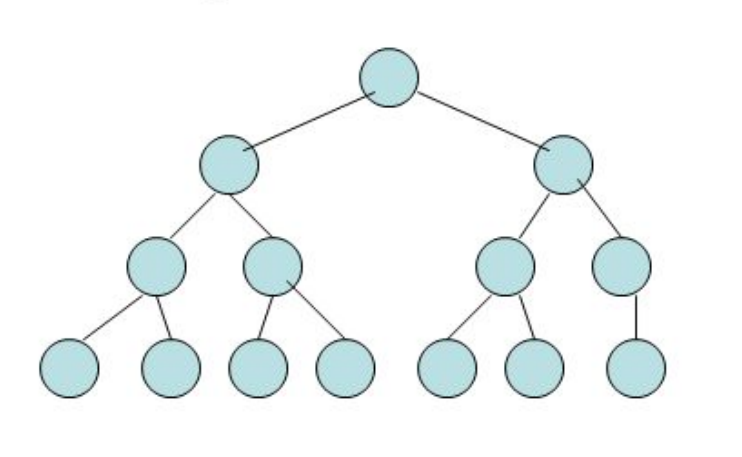
\includegraphics[width=\textwidth]{APB} 
        \caption{È un APB}
    \end{subfigure}
    \hfill
    \begin{subfigure}[b]{0.45\textwidth}
        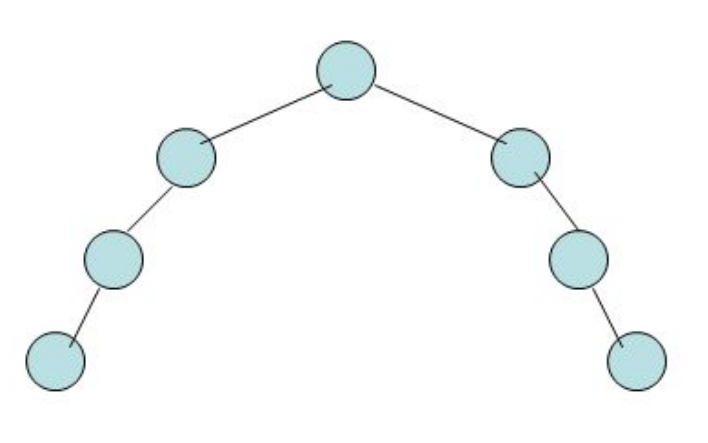
\includegraphics[width=\textwidth]{NAPB} 
        \caption{NON è un APB}
    \end{subfigure}
    %\caption{Didascalia generale per entrambe le immagini}
\end{figure}


\subsection{Alberi AVL}
Gli alberi AVL sono particolare tipi di albero binario di ricerca in cui vale la seguente condizione:
$$ | h(T->sx) - h(|T->dx) |  \le 1 $$ 
Quindi l'altezza del sottoalbero sinistro di T e quella del sottoalbero destro di T differiscono al più di uno, ovviamente si applica ad ogni sottonodo.\\
A differenza degli alberi perfettamente bilanciati, non si pone un limite sulla cardinalità dell'insieme ma bensi sull'\textbf{altezza} dei sottoalberi.\\

\begin{figure}[H]
    \centering
    \begin{subfigure}[b]{0.45\textwidth}
        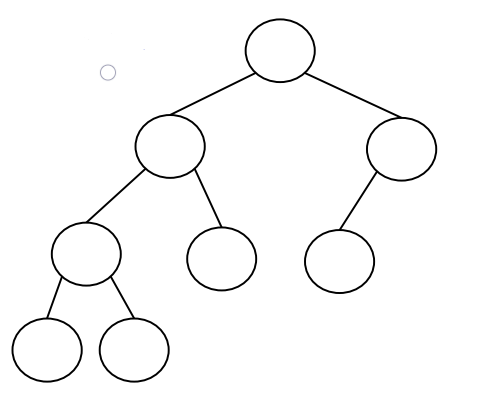
\includegraphics[width=\textwidth]{AVL} 
        \caption{È un AVL}
    \end{subfigure}
    \hfill
    \begin{subfigure}[b]{0.45\textwidth}
        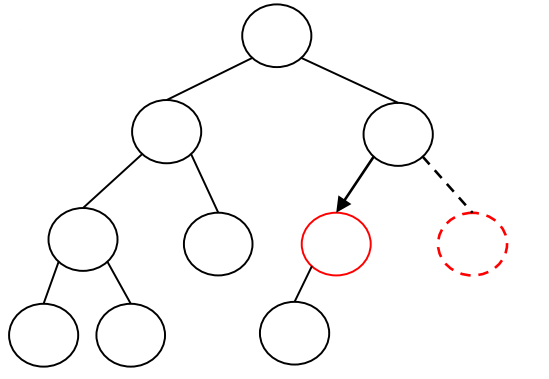
\includegraphics[width=\textwidth]{NAVL} 
        \caption{NON è un AVL}
    \end{subfigure}
    %\caption{Didascalia generale per entrambe le immagini}
\end{figure}
\begin{center}
    \textbf{Un albero pieno è sia ABL che AVL}    
\end{center}

\subsection{Alberi AVL Minimi}
Fissato $h$, l'albero AVL minimo di altezza $h$ è l'albero AVL di altezza $h$ col minor numero di nodi possibile.\\
Per ogni altezza andiamo a mostrare un possibile albero:

\begin{figure}[H]
    \centering
    \begin{subfigure}[b]{0.35\textwidth}
        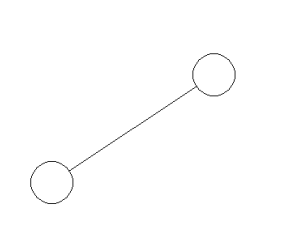
\includegraphics[width=\textwidth]{AVLh1} 
        \caption{AVL minimo di altezza 1}
    \end{subfigure}
    \hfill
    \begin{subfigure}[b]{0.45\textwidth}
        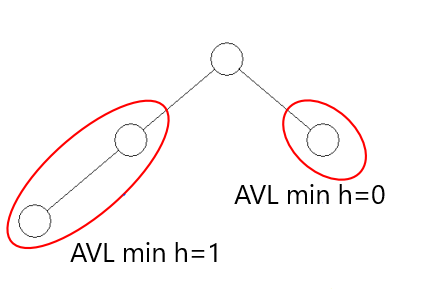
\includegraphics[width=\textwidth]{AVLh2} 
        \caption{AVL minimo di altezza 2}
    \end{subfigure}
    \hfill
    \begin{subfigure}[b]{0.45\textwidth}
        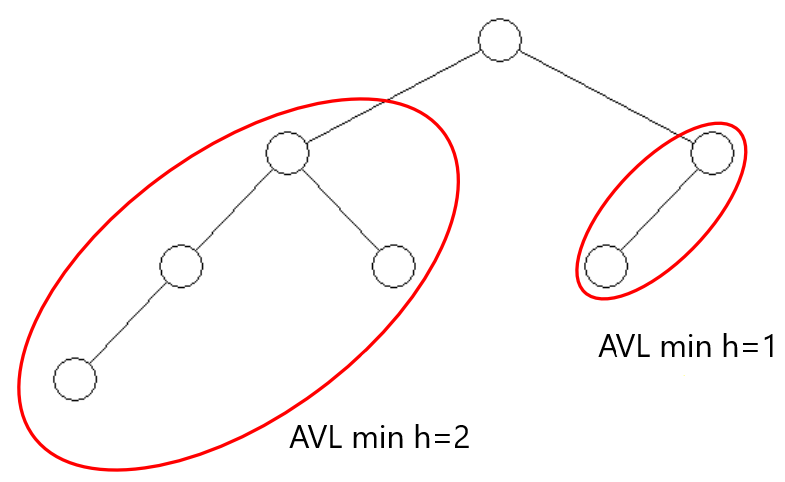
\includegraphics[width=\textwidth]{AVLh3} 
        \caption{AVL minimo di altezza 3}
    \end{subfigure}
    \hfill
    \begin{subfigure}[b]{0.45\textwidth}
        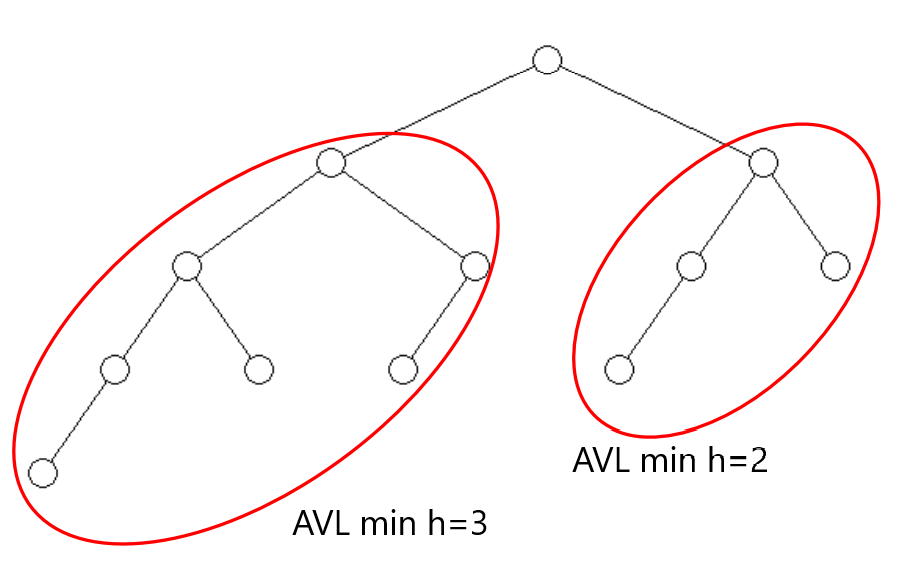
\includegraphics[width=\textwidth]{AVLh4} 
        \caption{AVL minimo di altezza 4}
    \end{subfigure}
\end{figure}
Possiamo notare un certo pattern che si ripeto, nello specifico dato un albero di altezza $h$ il sottoalbero sinistro sarà $h-1$ e il ciaosottoalbero destro $h-2$.\\
Andiamo a generalizzare questa osservazione:
$$ N(h)= \begin{cases}
    h+1 & \text{se } h=0,1\\
    1+N(h-1)+N(h-2) & \text{e poniamo per assurse } h \ge 2
\end{cases} $$
\textbf{DIM $h \ge 2$:}\\
Prediamo un generico AVL $T$ minimo, e poniamo per assurdo che il suo sottoalbero sinistro \textbf{è un AVL non minimo}, dunque esisterà un albero $T^{\prime}$ con sottoalbero sinistro che sarà \textbf{AVL minimo}. Quindi è un assurdo il fatto che esisterà un sottoalbero di $T^{\prime}$ di altezza $h-1$ con un numero minore di nodi rispetto al sottoalbero di $T$. In generale dunque se andiamo a dire che $T$ è un Albero AVL minimo, non è possibile che esiste un $T^{\prime}$ con un numero di nodi \textbf{minore} di un albero AVL minore.

Data la formula precendete facciamo una considerazione:\\
\begin{center}
    \begin{tabular}{|c|c|c|c|c|c|c|c|c|c|} % Sostituisci 'c' con 'l' se vuoi l'allineamento a sinistra
        \hline
        Altezza & 0 & 1 & 2 & 3 & 4 & 5 & 6 & 7 & 8 \\
        \hline
        Numeri Nodi & 1 & 2 & 4 & 7 & 12 & 20 & 33 & 54 & 88 \\
        \hline
        Fibonacci & 0 & 1 & 1 & 2 & 3 & 5 & 8 & 13 & 21 \\
        \hline
    \end{tabular}
\end{center}

Possiamo notare come ci siamo un certo collegamento tra i numeri di nodi e la sequenza di fibonacci, nello specifico notiamo come:
$$ N(h) = F(h+3)-1$$
Facciamo un ragionamento su come ricaverci l'altezza dato  la formula chiusa di Fibonacci:
$$ F(x)= \frac{1}{\sqrt{5}} [(\frac{1+\sqrt{5}}{2})^x - \cancel{(\frac{1-\sqrt{5}}{2})^x}]  $$
Andiamo a rimuovere la seconda parte poiché tende a zero.\\
$$ F(x)=c \cdot k^x $$
$$ N(h) = F(h+3)-1 $$
$$ N(h) = c \cdot k^{h+3}-1$$
$$ \frac{N(h)-1}{c} = k^{h+3} $$ 
$$ h =  \log_k (\frac{N(h)-1}{c}) -3 $$
Abbiamo dimostrato che l'altezza è logaritmica sul numero di nodi.\\
Adesso andiamo a dimostrare che la formula dei nodi vale per ogni $h$\\
\textbf{DIM:}
\begin{itemize}
    \item \textbf{Caso base:} $N(0) = F(0+3) - 1 = 1$
    \item \textbf{Caso induttivo:}
    \[
    N(h) = 1 + N(h-1) + N(h-2)
    \]
    Per ipotesi:
    \[
    N(h-1) = F(h+2) - 1
    \]
    \[
    N(h-2) = F(h+1) - 1
    \]
    Quindi:
    \[
    1 + (F(h+2) - 1) + (F(h+1) - 1) = F(h+3) - 1
    \]
\end{itemize}

\section{Lezione 11 - 14/04/2023}

\subsection{Operazioni di Riga riguarda il Determinante}
Le operazioni di riga preservano la non nullità del determinante ma non il valore.
\begin{itemize}
\item[$E_1$]: Scambiare due rige fa cambiare il segno
\item[$E_2$]: Bisogna moltiplicare per uno scalare anche il determinante (da rivdere)
\end{itemize}

\subsection{Determinante di una Matrice a Gradini}
Il modo più semplice per riusciure a calcolare il determinante di una matriace è portarla a gradini, poiché il determinante è \textbf{il prodotto della diagonale principale}.\\
$$ 
\begin{pmatrix}
1 & 0 & 0 \\
0 & 2 & 2 \\
0 & 0 & 3
\end{pmatrix} 
\Rightarrow det = 1*2*3 = 6 \Rightarrow Indipendente
$$

\subsection{Invertilità di una Matrice}
Presa una matrice $A \in \mathbb{R}_{n,n}$ esiste una matrice $B \in R_{n,n}$ tale che:
$$ AB = I_n = BA $$
Vale solo se il determinante è diverdo da zero.
$$ |A| \neq 0 \Leftrightarrow \exists inversa B=A^{-1} $$
$A^{-1}$ è unica.
Dim unicità:
$$ B_1=B_1I_N=B_1(AB_2)=(B_1A)B_2=I_nB_2=B_2 $$
Dim $\Rightarrow$:
$$ AB = I_n \Rightarrow det(AB) = det(I_n) = 1 $$
Dim $\Leftarrow$:
TODO:FINIRE

\subsection{Minore di una Matrice (sottomatrice quadrata)}
Indichiamo il minore come:
$$ A_{(i_1,...,i_h; j_1,...,j_n)} $$
\begin{itemize}
\item[]$i_1,...,i_h$ indica le righe
\item[]$j_1,...,j_n$ indica le colonne
\end{itemize}
Consideriamo la seguente matrice:
$$
\begin{pmatrix}
2 & 3 & 0 \\
0 & 1 & 2 \\
1 & 0 & 0
\end{pmatrix}
$$
$$ A_{(2,3;2,3)} = \begin{pmatrix}
1 & 2\\
0 & 0
\end{pmatrix} $$
I minori valgono anche sulle matrice rettangolari ma i minori rimangono sottomatrici quadrate.\\

\subsection{Grado Massimo}
Un minore si dice di \textbf{grado massimo} se il suo grado coincide con $min\{n,m\}$.\\
Una matrice non quadrata ha sempre più di un minore di ordine massimo, mentre una matrice quadrata ha un solo minore di ordine massimo ed è la matrice stessa.
\subsubsection{Esempio}
$$
\begin{pmatrix}
1 & 1 & 1 & 1 \\
2 & 2 & 2 & 2 \\
0 & 0 & 1 & 1 
\end{pmatrix}
$$
Consideriamo:
$$ A_{(2,3;2,4)} = \begin{pmatrix}
2 & 2 \\ 0 & 1
\end{pmatrix}$$
Questo non di grado massimo poichè il grado massimo è $min\{3,4\} = 3$

\subsection{Orlato}
Se abbiamo un minore che non è di grado massimo, possiamo orlarlo aggiungendo una riga e una colonna.\\
Un orlato rimane un minore, e si più orlare un orlato.\\
Riprendiamo l'esempio di sopra, eravamo rimasti che $A_{(2,3;2,4)}$ non fosse di grado massimo, andiamo ad orlarlo:
$$ A_{(1,2,3;2,3,4)} = \begin{pmatrix}
1 & 1 & 1 \\
2 & 2 & 2 \\
0 & 1 & 1 \\
\end{pmatrix} $$
Abbiamo raggiunto una matrice di grado massimo orlando cioè abbiamo aggiunto la $1$ riga e la $3$ colonna.

\subsection{Minore Fondamentale}
Si definisce \textbf{minore fondamentale} un minore che rispetta queste propietà:
\begin{itemize}
\item[1)] $det \neq 0$
\item[2)] Tutti i suoi orlati hanno $det = 0$  
\end{itemize}
\textbf{ESISTONO SEMPRE I MINORI FONDAMENTALI}\\
Non ci sono sempre minori fondamentali, ad esempio la matrice nulla non ha minori fondamentali, ma, se la matrice non è nulla allora esiste sempre almeno un minore fondamentale. Il minore fondamentale non è necessariamente unico.\\
Se un minore di ordine massimo ha determinante diverso da zero allora esso è un minore fondamentale

\subsubsection{Algoritmo per trovare Minore Fondamentale}
Un modo semplice per trovare un \textbf{minore fonmentale} è cominciare sempre da un minore molto piccolo e poi andare ad orlarlo fino a raggiugere il grado massimo.\\
Cominciamo con prendere una matrice:
$$ \begin{pmatrix}
1 & 1 & $\hlcyan{1}$ & 0 \\
2 & 3 & 4 & 0 \\
1 & 1 & 1 & 0 
\end{pmatrix} $$
Andiamo a prendere un minore "piccolo" con determinante diverso da zero:
$$ A_{(1;3)} = (1) \; \text{con det} \neq 0 $$
Abbiamo escludo gli "zeri" poiché il loro determinante è zero.\\
Procediamo con nostro "algoritmo" andando ad orlarlo:
$$ A_{(1;3)} \rightarrow A_{(1,2;3,4)} = \begin{pmatrix} 1 & 0 \\ 4 & 0 \end{pmatrix} det = 0 $$
Avendo trovato $det = 0 = (1*0)-(0*4)$ dobbiamo scegliere un altro orlato:
$$ A_{(1;3)} \rightarrow A_{(1,2;2,3)} = \begin{pmatrix} 1 & 1 \\ 3 & 4 \end{pmatrix} det = 1 $$
Abbiamo raggiunto un buon candidato ora dobbiamo vericare che tutti i suoi orlati abbiano $det = 0$, in questo caso il suo unico orlato è:
$$ A_{(1,2;3,4)} \rightarrow A_{(1,2,3;1,2,3)} = \begin{pmatrix}
 1 & 1 & 1 \\
 1 & 3 & 4 \\
 1 & 1 & 1
\end{pmatrix} \; \text{ unico orlato con }  det=0$$
Quindi in definitiva:
$$ A_{(1,2;2,3)} = \begin{pmatrix} 1 & 1 \\ 3 & 4 \end{pmatrix} $$ 
$$ \textbf{MINORE FONDAMENTALE}$$

\subsection{Teorema degli Orlati (NO DIM)}
Sia $A \in \mathbb{R}_{n,m} $ matrice rettangolare e $A(i_1,...,i_h; j_1,...,j_n)$ minore fondamentale allora $\Rightarrow$:
$$ \underline{a}_{1,1},...,\underline{a}_{i,n}$$
Sono una base dello spazio vettoriale generato dalle \textbf{righe}.\\
(Esiste equivalente per colonne)
Conseguanza di ciò:
$$ \textbf{dim Righe Generate = dim Colonne Generate} $$

\subsubsection{Rango}
$$ \textbf{Rango = dim(Minore Fondamentale)} $$
Da questo sappiamo che i pivot di una matrice a gradini corrisponde alla dimensione, quindi al \textbf{rango}.

\subsubsection{Corollari derivati}
\begin{itemize}
\item[•] Il rango di riga è sempre uguale al rango di colonna, inoltre il rango di $A$ è uguale al numero di pivot di una matrice a gradini equivalente per righe.
\item[•] Tutti i minori fondamentali hanno lo stesso grado
\item[•] Il determinante di una matrice quadrata è diversa da zero se e solo se le righe (o colonne) sono indipedenti
\item[•] $det A = 0 \Leftrightarrow \; \text{righe (o colonne) dipendenti}$
\end{itemize}

\subsection{Criteri di compatibilità sistemi di equazioni lineare}
Consideriamo un sistema lineare:
$$
\syssubstitute{A{a_{11}}B{a_{21}}C{a_{m1}}D{a_{1n}}E{a_{2n}}F{a_{mn}}X{x_{n}}}
\systeme{
  A x_1 +...+ D X  = c_1,
  B x_1 +...+ E X = c_2,
  C x_1 +...+ F X = c_n
}
$$
Possiamo scriverlo in forma matrice nel seguenti modo $AX=C$:
$$ A = \begin{pmatrix} a_{11} & \dots & a_{1n} \\ \vdots & \ddots & \vdots \\ a_{n1} & \dots & a_{n1} \end{pmatrix} \; X = \begin{pmatrix} x_1 \\ \vdots \\ x_n \end{pmatrix} \; C =  \begin{pmatrix} c_1 \\ \vdots \\ c_n \end{pmatrix} $$
Possiamo esprimere per $C$ e spezzarla:
$$ 
C = x_1 \begin{pmatrix} a_{11} \\ \vdots \\ a_{n1} \end{pmatrix} +...+ x_n \begin{pmatrix} a_{1m} \\ \vdots \\ a_{nm} \end{pmatrix}
$$
Quindi se c’è una soluzione la colonna dei termini noti quindi se c’è una soluzione la colonna dei termini noti.\\
\subsubsection{Primo Criterio di Compatibilità}
Un sistema S  è compatibile $\Leftrightarrow$ la colonna dei termini noti è combinazione lineare della matrice incompleta (è soluzione).







\section{Lezione 12 - 19/04/2023}

\subsection{Teorema di Rouché-Capelli}
Il teorema di Rouché-Capelli anche noto come secondo sistema di compatibilità afferma che un sistema $S$ è compatibile $\Leftrightarrow$ il rango della matrice incompleta è uguale al rango della matrice completa.
$$
\syssubstitute{A{a_{11}}B{a_{21}}C{a_{m1}}D{a_{1n}}E{a_{2n}}F{a_{mn}}X{x_{n}}}
\systeme{
  A x_1 +...+ D X  = c_1,
  B x_1 +...+ E X = c_2,
  C x_1 +...+ F X = c_n
}
\; \text{è compatibile} \Leftrightarrow
v(A) = v(A^{\prime})
$$

\textbf{DIM $\Rightarrow$:}
Per il primo principio compatibilità:
$$ 
\begin{pmatrix}
c_1 \\ \vdots \\ c_n
\end{pmatrix}
=
y_1 \begin{pmatrix}
a_{11} \\ \vdots \\ a_{n1}
\end{pmatrix}
+...+
y_n \begin{pmatrix}
a_{1m} \\ \vdots \\ a_{nm}
\end{pmatrix}
$$
$$ (c_1,...,c_n) \; \text{DIPENDE DALLE COLONNE}$$
DA FINIRE
\textbf{DIM $\Leftarrow$:}
Partiamo da "i due ranghi sono uguali" allora per il teorema degli orlati hanno lo stesso ordine/grado $(L)$.\\
Consideriamo una matrice:
$$
\begin{pmatrix}
a_{11} & \dots & a_{1n} &\aug& c_1 \\
\vdots & \ddots & \vdots &\aug& \vdots \\
a_{n1} & \dots & a_{nm} &\aug& c_n 
\end{pmatrix}
$$
Consideriamo un minore fondamentale della matrice incompleta (base), ma dalla ipotesi lo è anche per la matrice completa.\\
Allora per il teorema degli orlati: le colonne del minore fondamentale formano un sistema di generatori di tutta la matrice allora il sistema è compatibile-

\subsubsection{Esempio Parametrico}
Consideriamo il seguente sistema:
$$ 
\systeme{
x+y+zh = 2,
2x+3y+z = 1,
x+5y+z = 0
}
$$
Abbiamo un fattore \textbf{parametrico} cioé $h$, vogliamo sapere per quali valori di $h$ il sistema è compatibile:\\
Potremmo procedere con la risoluzione a gradini ma ci viene più facile con Rusché-Capelli, costruiamo la matrice:
$$ 
\begin{pmatrix}
1 & 1 & h & \aug & 2 \\
2 & 3 & 1 & \aug & 1 \\
1 & 5 & 1 & \aug & 0
\end{pmatrix}
$$
Comincio a trovare il minore fondamentale della matrice incompleta, come sempre iniziamo dal "basso" quindi consideriamo $1$ nella posizione $3;1$ e andiamo ad orlarlo:
$$
A(2,3;1,2) = 
\begin{pmatrix}
2 & 3 \\
1 & 5
\end{pmatrix}
$$
Dalla definizione di minore fondamentale abbiamo bisogno che il suo determinante sia diverso da zero ($2*5-1*3 \neq 0$) e che tutti i suoi orlati abbiano determinante uguale a 0, in questo caso l'unico orlato possibile (della matrice incompleta) è:
$$
A(1,2,3;1,2,3) = 
\begin{pmatrix}
1 & 1 & h \\
2 & 3 & 1 \\
1 & 5 & 1
\end{pmatrix}
$$
Per calcolare il determinante usiamo $Sorrus$ ci verrà:
$$ 3+1+10h - 3h-2-5 = 7h-3 $$
Essendo che il determinante è anch'esso parametrico abbiamo due casi:
\begin{itemize}
\item[] SE $h=\frac{3}{7}$ allora il $det = 0$ quindi il rango sarà $2$
\item[] SE $h \neq \frac{3}{7}$ allora il $det \neq 0$ quindi il rango sarà $3$
\end{itemize}
(Ovviamente nel caso $h \neq \frac{3}{7}$ il minore fondamentale è la matrice stessa)
Ora dobbiamo trovare il rango della matrice completa, come sempre dobbiamo trovare un minore fondamentale:
$$ 
A(1,2,3;1,2,4) =
\begin{pmatrix}
1 & 1 & 2 \\
2 & 3 & 1 \\
1 & 5 & 0
\end{pmatrix}
$$
Il determinante è diverso da zero quindi è un minore fondamentale, quindi il rango della matrice completa è $3$.\\
Per il teorema di Rusché-Capelli il sistema è compatibile se e solo se il rango delle due matrice combacia ma essendo il rango della matrice incompleta parametrico abbiamo due casi:
\begin{itemize}
\item[]SE $h = \frac{3}{7}$ $ 3 \neq 2 $ INCOMPATIBILE
\item[]SE $h \neq \frac{3}{7}$ $ 3 \neq 3 $ COMPATIBILE (rango massimo)
\end{itemize}
Sappiamo che per $h \neq \frac{3}{7}$ il sistema è compatibile ora bisogna trovare le soluzioni, usiamo la seguente tecnica:
$$ AX=C $$
Sappiamo che $A$ ha determinante diverso da zero allora è invertibile allora sfruttando quello che abbiamo visto a 9.3, sappiamo che le soluzioni $X=A^{-1}C$, allora:
$$ 
A^{-1} =  \frac{1}{7h-3} 
\begin{pmatrix}
A_{11} & A_{21} & A_{31} \\
A_{12} & A_{22} & A_{32} \\
A_{13} & A_{23} & A_{33}
\end{pmatrix}
$$
Ricordiamo che $A_{11}...$ sono i complementi algebrichi.
$$ 
A^{-1} =
\begin{pmatrix}
-2 & 1-h5 & 1-3h \\
1 & 1h & 1*2h \\
7 & 4 & 1
\end{pmatrix}
$$
Quindi ora possiamo esprimere $X$ come:
$$
X = \begin{pmatrix}
X \\ X \\ X
\end{pmatrix}
=
\begin{pmatrix}
-2 & 1-h5 & 1-3h \\
1 & 1h & 1*2h \\
7 & 4 & 1
\end{pmatrix}
*
\begin{pmatrix}
2 \\ 1 \\ 0
\end{pmatrix}
$$

\subsection{Regola di Cramer}
La Regola(Metodo) di Cramer ci dà una mano nel trovare le soluzione di sistema di equazione di \textbf{n equazione, n incognite}.\\
Se ci sono $n$ equazioni ed $n$ incognite sappiamo che la matrice
incompleta è una matrice quadrata, e poiché le righe della matrice quadrata sono indipendenti poiché fanno sempre parte del minore fondamentale, la matrice $A$ ha determinante diverso da zero, questo implica che possiamo invertirla, quindi:
$$ AX=C \Rightarrow X=A^{-1}C $$
Esperiamiamo:
$$ 
\begin{pmatrix}
X_1 \\ \vdots \\ X_n
\end{pmatrix}
= 
\frac{1}{detA = |A|}
\begin{pmatrix}
A_{11} & A_{21} & \dots & A_{n1} \\
A_{12} & \ddots & \dots & \vdots \\
A_{1m} & A_{23} & \dots & A_{nm}
\end{pmatrix}
\begin{pmatrix}
C_1 \\ \vdots \\ C_n
\end{pmatrix}
=
$$
$$ 
=
\begin{pmatrix}
C_1A_{11}+C_2A_{21}+...+C_nA_{n1} \\
\vdots \\
C_1A_{1m}+C_2A_{2m}+...+C_nA_{nm} 
\end{pmatrix}
$$
Infine dalla eguaglianza:
$$ x_1 = \frac{c_1A_{11}+...+c_nA_{n1}}{|A|} $$
%$$ \; \vdots $$
$$ x_n = \frac{c_1A_{1n}+...+c_nA_{nm}}{|A|} $$

\subsubsection{Metodo Semplificato}
Un metodo più semplice prevede di far utilizzo di una matrice ausiliaria andando a sostituire alla $i$-sima colonna i termini noti.\\
Nello specifico se vogliamo calcolarci $x_1$ andremo a sostituire alla prima colonna, la colonna dei termini noti in questo modo:
$$
B_1 = 
\begin{pmatrix}
c_{11} & a_{12} & \dots & a_{1n} \\
c_{21} & \ddots & \vdots & \vdots \\
\vdots & \vdots & \ddots & \vdots \\
c_{n1} & \dots & \dots & a_{nn}
\end{pmatrix}
$$
Ne consegue che a $B_2$ andrà sostituita la seconda colonna e così via...\\
Tornando a $B_1$ se andiamo a calcolare il determinante della prima colonna (che è anche il determinante della matrice stessa) otteremo:
$$ c_1A_{11}+...+c_nA_{n1} $$
che è proprio il numeratore della regola di Cramer, quindi possiamo semplificare nel seguenti modo:
$$ x_1 = \frac{|B_1|}{|A|} $$

\subsubsection{Esempio}
Riprendiamo l'esempio di prima:
$$
(h \neq \frac{3}{7}) \; S =  
\systeme{
x+y+zh = 2,
2x+3y+z = 1,
x+5y+z = 0
}
$$
Dato che ci troviamo nella situazione di $n$ equazioni, $n$ incognite possiamo applicare Cramer, ci aiutiamo usando la matrice ausilaria:
$$ 
B_1 = 
\begin{pmatrix}
2 & 1 & h \\
1 & 3 & 1 \\
0 & 5 & 1 
\end{pmatrix} \; |B_1| = 5h-5
\; \; \; \; \; x_1 = \frac{5h-5}{7h-3} 
$$

$$
x_2 = \frac{h-1}{7h-3} 
$$

$$
x_3 = \frac{10}{7h-3} 
$$










\section{Lezione 13 - 13/04/2023}

\subsection{Esempio Moneta}

\section{Lezione 14 - 26/04/2023}

\subsection{Propietà}
Consideriamo una funzione lineare $f: V \rightarrow W$ elenchiamo le seguenti propietà:

\begin{itemize}


\item[1)] $f(\underline{0}_v) = \underline{0}_w$


\item[2)] $f(h_1\underline{v}_1+...+h_n\underline{v}_n) = h_1f(\underline{v}_1)+...+h_nf(\underline{v}_n)$


\item[3)] $\underline{v} \; \text{dipende da} \; \underline{v}_1,...,\underline{v}_n \Rightarrow f(\underline{v}) \; \text{dipende da} \; f(\underline{v}_1),...,f(\underline{v}_n)$\\
$\textbf{DIM:}$
$$ \underline{v} = h_1\underline{v}_1+...+h_n\underline{v}_n $$
$$ f(\underline{v}) = f(h_1\underline{v}_1+...+h_n\underline{v}_n) =^{2)} h_1f(\underline{v}_1)+...+h_nf(\underline{v}_n)$$

\item[3.1)] $f$ conserva dipendenza lineare MA NON L'INDIPENDENZA
$$ \underline{v}_1,...,\underline{v}_n \;DIP\; \Rightarrow f(\underline{v}_1),...,f(\underline{v}_n) \;DIP\; $$
$$ \exists \underline{v}_i \;DIP\; \underline{v}_1,...,\underline{v}_{i+1},...,\underline{v}_n \Rightarrow f(\underline{v}_i) \;DIP DA\; f(\underline{v}_1),...,f(\underline{v}_{i+1}),...,f(\underline{v}_n)$$

\item[4)] $f(<S>) = <f(S)> = <f(\underline{v}_1),...,f(\underline{v}_n))>$\\

Andiamo a dimostare la prima uguaglianza nel solito modo:
\subitem DIM $\subseteq$:
$$ \underline{v} \in f(<S>) $$
$$ \exists \underline{w} \in <S> \underline{v} = f(\underline{w})$$
$$ \underline{w} = h_1\underline{v}_1+...+h_n\underline{v}_n$$
$$ f(\underline{w}) = h_1f(\underline{v}_1)+...+h_nf(\underline{v}_n) \in <f(S)>$$
 
\subitem DIM $\supseteq$:
$$ \underline{w} \in <f(S)> $$
$$ \underline{w} = h_1f(\underline{v}_1)+...+h_nf(\underline{v}_n)$$
$$ f(h_1\underline{v}_1+...+h_n\underline{v}_n) \in f(<S>)$$
$$ \underline{w} \in f(<S>) $$

\item[5)] $H \le V \rightarrow f(H) \le W$\\
Dimostriamo sia sottospazio vettoriale:

\subitem Non vuoto:
$$ \underline{0} \Rightarrow f(\underline{0})= \underline{0} \in H $$
\subitem Stabilità Somma:
$$ \underline{w},\underline{w}^{\prime} \in f(H) \;\;\;\;\; \underline{v},\underline{v}^{\prime} \in H $$
$$ \underline{w} = f(\underline{v}) \;\;\;\;\; \underline{w}^{\prime} = f(\underline{v}^{\prime}) $$
$$ \underline{w}+\underline{w}^{\prime} = f(\underline{v})+f(\underline{v}^{\prime})= f(\underline{v}+\underline{v}^{\prime}) \in f(H) $$

\subitem Stabilità Prodotto:
TODO: DA FARE COME ESERCIZIO (un giorno lo farò)

\end{itemize}

\subsection{Kernel}

Consideriamo la funzione lineare $f: V \rightarrow W$, denotiamo con $Im f$ il sottospazio immagine di $f$ cioé: $\{f(\underline{v})/\underline{v} \in V\}=f(V) = Im f$.\\

Andiamo a definire un altro insieme chiamato \textbf{Kernel} o anche detto \textbf{ker}, cioé l'insieme di tutti i valori del dominio che vanno a finire nel neutro nella fattispecie: $ ker f = {\underline{v} \in V / f(\underline{v}) = \underline{0}} $\\

Andiamo a dimostare che il ker sia un sottospazio:
\begin{itemize}
\item[Non vuoto:] Vero poiché il neutro gli appartiene

\item[Stabilità Somma:]
$$ \underline{v},\underline{v}^{\prime} \in ker f \Rightarrow \underline{v}+\underline{v}^{\prime} \in ker f $$

$$ f(\underline{v})+f(\underline{v}^{\prime}) = f(\underline{v}+ \underline{v}^{\prime}) = \underline{0}+\underline{0} = \underline{0} $$

\item[Stabile Prodotto:]
$$ h \in \mathbb{R} \;\;\;\;\; h\underline{v} \in ker f$$
$$ f(h\underline{v}) = hf(\underline{v}) = \underline{0} $$

\end{itemize}

Avendo definito questi due concetti possiamo sfruttare alcune propietà per capire più facilente l'iniettività o surriettività di un applicazione lineare:
\begin{itemize}
\item[•] Se l'immagine del dominio combacia col codominio allora la funzione \textbf{è surriettivita}
$$ f(V) = Im f = W \Leftrightarrow \text{f è surriettiva} $$

\item[•] Se il $ker f = \{\underline{0}\} \Leftrightarrow$ $f$ è \textbf{iniettiva.}\\

\subitem \textbf{DIM $\Rightarrow$:}
$$ \underline{v},\underline{w} \in V \; \text{con} \; f(\underline{v}) = f(\underline{w}) \Rightarrow \underline{v} = \underline{w} $$
$$ f(\underline{v}-\underline{w}) = f(\underline{v})-f(\underline{w}) = \underline{0} \Rightarrow \underline{v}-\underline{w} \in ker f \Rightarrow \underline{v}-\underline{w} = \underline{0} \Rightarrow \underline{v} = \underline{w}$$

\subitem \textbf{DIM $\Leftarrow$:}
$$ \underline{0} \in ker f \;\;\;\;\; \{\underline{0}\} \subseteq ker f $$
$$ \underline{v} \in ker f \Rightarrow f(\underline{v}) = \underline{0} \Rightarrow \underline{v} = \underline{0} $$
Tutti gli elementi combaciano con il neutro

\end{itemize}


\subsubsection{Esempi}
\begin{itemize}
\item[•] $\underline{0}_v: V \rightarrow V (\underline{v} \rightarrow \underline{0})$\\
$$ Im f = f(V) = \{\underline{0}\} $$
$$ Ker f = V$$ 
$$ \text{INIETTIVA E SURRIETTIVA } \Leftrightarrow V = \{\underline{0}\}$$

\item[•] $ id_v V \rightarrow V (\underline{v} \rightarrow \underline{v})  $
$$ Im f = f(id_v) = V \; INIETTIVA$$
$$ Ker f = \{\underline{0}\} \;  SURRIETTIVA$$

\item[•] $\mathbb{R}^2 \rightarrow \mathbb{R}^2$
$$ (x,y) \rightarrow \begin{pmatrix}1 & 2 \\ 0 & 1\end{pmatrix} \begin{pmatrix}x \\ y \end{pmatrix} = \begin{pmatrix}x+2y \\ y\end{pmatrix} $$

\subitem • Per verificare l'iniettività dobbiamo verificare il $ker f$ sia formato solo dal vettore nullo, quindi vediamo per quali valori di $x,y$ $f(x,y) = 0$:
$$ \systeme{x+2y=0, y=0} \Rightarrow \systeme{x=0,y=0} \; \text{È INIETTIVA} $$

\subitem • Per verificare la surrietività prendiamo un sistema di generatori, in questo caso quella canonica:
$$ <(1,0),(0,1)> \; dim=2$$
$$ f(\mathbb{R}^2) = <f(1,0),f(0,1)> = <(1,0),(2,1)>$$
Essendo indipendenti hanno $dim=2$ quindi è surriettiva visto che è rimasto un sistema di generatori.

\item[•] $f: \mathbb{R}_2[x] \rightarrow \mathbb{R}[x] (ax^2+bx+c \rightarrow 2ax+b)$\\

\subitem •  Per verificare l'iniettività dobbiamo verificare il $ker f$ sia formato solo dal vettore nullo, quindi vediamo per quali valori di $a,b,c$ $f(ax^2+bx+c) = 0$:
$$ \underline(v) \in \mathbb{R}_2[x] / f(\underline{v})= \underline{0}$$
$$ f(ax^2+bx+c) =  2ax+b = \underline{0} \Leftrightarrow a = 0 = b $$
Quindi per $ker f$ sarà formato da tutti i valori $c \in \mathbb{R}$ quindi non è iniettiva.
$$ ker f = \{c/c \in \mathbb{R}\} DIM=1$$

\subitem •  Per verificare la surrietività prendiamo un sistema di generatori, in questo caso quella canonica:
$$ <x^2,x,1> dim=3$$
$$ f(<x^2,x,1>) = <2x,1,0> = <2x,1> dim = 2 \; \textbf{NON È SURRIETIVA}$$

\item[•] $f: \mathbb{R}^2 \rightarrow \mathbb{R}^3 $
$$ (x,y) \rightarrow \begin{pmatrix} 1&2\\3&4\\0&1 \end{pmatrix} \begin{pmatrix} x \\ y \end{pmatrix} $$

\subitem •  Per verificare l'iniettività dobbiamo verificare il $ker f$ sia formato solo dal vettore nullo, quindi vediamo per quali valori di $x,y$ $f(x,y) = 0$:
$$ \begin{pmatrix} 1&2\\3&4\\0&1 \end{pmatrix} \begin{pmatrix} x \\ y \end{pmatrix} = \begin{pmatrix} 0 \\ 0 \end{pmatrix}  \Leftrightarrow \systeme{x+2y=0, 3x+4y=0, y=0} \Leftrightarrow \systeme{x=0,y=0} $$

\end{itemize}

\subsection{Altre propriepietà}
Consideriamo una generica funzione lineare $f: V \rightarrow W$:
\begin{itemize}
\item[•] Il monomorfismo (omomorfismo iniettivo) mantiene l'indipendenza, cioè:
$$  \underline{v}_1,...,\underline{v}_n \; INDIP. \Rightarrow f(\underline{v}_1),...,f(\underline{v}_n) \; INDIP.$$
$$ \text{BASE DI V} \rightarrow \text{BASE DI }f(V) $$
\textbf{DIM:}
Prendiamo una combinazione lineare dei vettori immagine ed eguagliamola all’elemento
neutro:
$$ f(h_1\underline{v}_1+...+h_n\underline{v}_n) = h_1f(\underline{v}_1)+...+h_nf(\underline{v}_n) = \underline{0}   $$
Possiamo leggerlo anche nel seguente modo:
$$ h_1\underline{v}_1+...+h_n\underline{v}_n \in ker f $$
Affinché questi vettori siano indipendenti bisogna dimostrare che tutti gli scalari siano necessariamente pari a zero ma essendo i vettori indipendenti per ipotesi ed avendolo uguagliato all'elemento neutro troviamo che tutti gli scalari sono nulli.

\item[•] $$ dim(ker f) + dim(Im f) = dim (V) $$ 
La dimensione del dominio è uguale alla somma delle dimensioni dell'immagine del dominio e del ker di f.\\
\textbf{DIM:}\\
Ragioniamo per casi:
\subitem • $ker f = \{\underline{0}\}$\\
Quindi la funzione ha $dim=0$ ed è iniettiva (monomorfismo) per quanto visto sopra conserva la base (indipendenza) e quindi la dimensione quindi:
$$ 0 + dim(Im f) = dim (V) $$

\subitem • $ker f = V$:\\
Come abbiamo dagli esempi di prima l'unico caso in cui $ker f = V$ è quando $f$ è la funzione nulla e sempre per la precendente osservezione $dim (Im f) = 0$, quindi:
$$ dim (ker f) + 0 = dim (V) $$

\subitem • $\{0\} < ker f < V$\\
\blindtext

\end{itemize}


\subsection{Cordinazione Associata}
Preso uno spazio vettoriale $V$ e un suo riferimento $(\underline{e}_1,...,\underline{e}_n)$ possiamo considerare la seguente funzione lineare:
$$ \underline{v} = h_1\underline{e}_1+...+h_n\underline{e}_n \rightarrow (h_1,...,h_n) \in \mathbb{R}^n $$




\section{Lezione 17 - 10/05/2023}

\subsection{Criteri di Diagonalizzazione}
Sia $f: V_n \rightarrow V_n$ un endomorfismo è diagonalizzabile $\Leftrightarrow$ $V_n$ ammette una base datta da autovettori.\\
\textbf{DIM $\Rightarrow$:}\\
Supponiamo esista un riferimento $\mathtt{R}$ e consideriamo la matrice associata:
$$ 
\exists \mathtt{R}=(\underline{e}_1,\underline{e}_2,...,\underline{e}_n): M_{\mathtt{R}}(f) = \begin{pmatrix}
a_1 & 0 & 0 \\
0 & \ddots & 0 \\
0 & 0 & a_n
\end{pmatrix}
$$
Andiamo fare l'immagini dei valori del riferimento come combinazione lineare rispetto le colonne
$$ 
f(\underline{e}_1) = a_1\underline{e}_1 + 0\underline{e}_2 + ...
f(\underline{e}_2) = a_2\underline{e}_2
...
f(\underline{e}_n) = a_n\underline{e}_n
$$
Quindi i valori del riferimento sono tutti \textbf{autovettori}.

\textbf{DIM $\Leftarrow$:}
Supponiamo quindi di avere un riferimento di autovettori
TODO: RIASCOLARE AUDIO


\subsection{Esercizio: Trovare gli autovalori}
Consideriamo il seguendo endomorfismo:
$$ f:\mathbb{R}^3 \rightarrow \mathbb{R}^3  $$
$$ (x,y,z) \rightarrow (-y,x,z) $$
Prendiamo un riferimento in questo caso quello canonico/naturale:
$$ \mathtt{R} = ((1,0,0),(0,1,0),(0,0,1)) $$
Costruiamoci la matrice associate delle immagini per colonna
$$ 
M_{\mathtt{R}} = \begin{pmatrix}
0 & -1 & 0 \\ 1 & 0 & 0 \\ 0 & 0 & 1 
\end{pmatrix}
$$
Andiamo a sotrarre la matrice diagonale con una variabile $t$:
$$ 
\begin{pmatrix}
-t & -1 & 0 \\ 1 & 0-t & 0 \\ 0 & 0 & 1-t 
\end{pmatrix}
$$
E andiamo a calcolarci il determinante 
$$ 
det (\begin{pmatrix}
-t & -1 & 0 \\ 1 & 0-t & 0 \\ 0 & 0 & 1-t 
\end{pmatrix}) 
= (1-t)(t^2+1) = 0
$$
Quello che ci siamo ricavati è il \textbf{polinomio caratteristico}, l'unica sua soluzione è:
$$ t = 1 \;\;\; \textbf{unico AUTOVALORES}$$

\subsubsection{Trovare Autovettore}
Avendo trovato che l'unico autovare è $t=1$ andiamo a sostiturlo nella matrice associata:
$$
\begin{pmatrix}
-1 & -1 & 0 \\ 1 & -1 & 0 \\ 0 & 0 & 0 
\end{pmatrix}
$$
Adesso andiamo a considerare il sistema di equazioni omogeneo:
$$ 
\begin{pmatrix}
-1 & -1 & 0 \\ 1 & -1 & 0 \\ 0 & 0 & 0 
\end{pmatrix}
\begin{pmatrix}
x \\ y \\ z
\end{pmatrix}
$$
$$
\systeme{-x-y=0, x-y=0, 0=0}
$$
Il sistema è già risolto e quindi l'insieme delle soluzioni è:
$$ 
S = \{(0,0,z)/ z \in \mathbb{R} \} = <(0,0,1)>
$$

\subsection{Autospazio relativo ad autovalore h}
Consideriamo il seguente endomorfismo $f: V_n \rightarrow V_n$ e $h$ un autovalore, definisco $V(h)$ lo \textbf{spazio relativo all'autovalore h}:
$$ V(h) = \{\underline{v}/f(\underline{v}) = h\underline{v}\} = 
\{\{\text{autovettori di autovalore h} \} \cup \{\underline{0}\} \} 
$$
È un sottospazio vettoriale (dimostazione da fare a casa :()
\subsubsection{Proprietà}
Elenchiamo le seguenti propietà:
\begin{itemize}
\item[•] $dim V(h) \ge 1 $ poiché c'è almeno un autovettore
\item[•] $V(h)$ isomorfo a $\{X/(A-\underbrace{hI_n}_{M_{\mathtt{R}}(f)})X=0 \} = \overline{S} $ mediante cordinazione associata
\item[•] Se $h \neq k$ allora $V(h) \cap V(k) = \{\underline{0}\}$\\
\textbf{DIM:}\\
Consideriamo $\underline{v} \neq \underline{0} \in  V(h) \cap V(k)$, allora può essere autovettore di autovalore di $h,k$, ma poiché un autovettore può avere un unico e solo autovalore si arriverebbe all’assurdo che $h = k$ quindi $\underline{v} = \underline{0}$ quindi l'intersezioni deve essere vuota.
\item[•] Se $\underline{v}_1,...,\underline{v}_n$ sono autovattore di autovalori $h_1,...,h_n$ autovalori \textbf{distinti}, allora sono \textbf{indipendenti}.\\
\textbf{DIM:}\\
Poniamo per assurdo che non siano indipendenti, allora questo vuol dire che:
$$ \underline{v}_1 = a_2\underline{v}_2+...+a_n\underline{e}_n $$
$$ f(\underline{v}_1) = h_1\underline{v}_1 $$
Sviluppiamo mantendendo l'uguaglianza:
$$ a_2f(\underline{v}_2)+...+.a_nf(\underline{v}_n) = h_1a_2\underline{v}_2+...+h_1a_n\underline{v}_n $$
$$ a_2h_2\underline{v}_2+...+a_nh_2\underline{v}_n = h_1a_2\underline{v}_2+...+h_1a_n\underline{v}_n $$
$$ a_ih_1 = a_ih_i $$ 
$$ h_1 = h_i$$
Siamo arrivando ad uno assurdo poiché distinti

\end{itemize}

\subsection{Corolarrio}
Consideriamo l'endomorfismo $f: V_n \rightarrow V_n$ allora:
$$ f \; \text{ammette n autovalori distinti} \rightarrow f \; \text{diagonalizzabile}  $$
\textbf{DIM:}\\
$$ \underline{v}_1,...,\underline{v}_n $$
Essendo distinti per quanto visto prima allora sono indipendenti, ma sempre per quanto osservato sono base di $V_n$, quindi è \textbf{diagonalizzabile}\\
\paragraph{Esempio}
Consideriamo $f: \mathbb{R}^3 \rightarrow \mathbb{R}^3$ quindi $n=3$
$$ (x,y,z) \rightarrow \begin{pmatrix}
2 & 0 & 0 \\ 1 & 3 & 0 \\ 0 & 0 & 1 
\end{pmatrix}
\begin{pmatrix}
x \\ y \\ z
\end{pmatrix} $$
Andiamo a calcolare il terminante andando a sottrarre alla diagonale $t$:
$$
det \begin{pmatrix}
2-t & 0 & 0 \\
1 & 3-t & 0 \\
0 & 0 & 1-t
\end{pmatrix}
= (1-t)(3-t)(2-t)
$$
Quindi le soluzioni del polinomio caratteristico sono $t=1,2,3$ essendo $3=n$ e distinti allora è \textbf{diagonalazzabile}

\subsection{Molteplicità Algebrica}
Considerato un generico polinomio:
$$ a_nx^n + a_{n-1}x^{n-1}+...+a_1x+a_0 = 0 $$
Per il teorema fondamentale dell'algebra:
$$ (x-c_1)...(x-c_n) \in \mathbb{C} $$
Possiano riscriverlo come:
$$ (x-c_1)^{n_1}...(x-c_n)^{n_m} $$
Quindi $n_i$ sarà la nostra molteplicità algebrica

\subsection{Relazione Moltiplicità Algebrica e Geometria}
Oltre la molteplicità algebrica che indicheremo con $m_a(h)$, defininiamo la \textbf{molteplicità Geometrica}, come la dimensione di uno \textbf{autospazio relativo ad h}:
$$ dimV(h) = m_g(h) $$
Inoltre fissiamo una relazione tra molteplicità algebrica e geometriaìca:
$$ 1 \le m_g(h) \le m_a(h) $$
\textbf{DIM:}\\
Prendiamo una base di $V(h)$ e completiamola a $V_n$s
$$ \underline{v}_1,...,\underline{v}_e \; \text{base di V(h)}$$
$$ \underline{v}_1,...,\underline{v}_e,...,\underline{v}_n \; \text{estesa a } V_n $$
Andiamo a prendere un riferimento:
$$\mathtt{R}=(\underline{v}_1,...,\underline{v}_e,...,\underline{v}_n)$$
E calcoliamo la matrice associata:
$$ M_{\mathtt{R}}(f) = 
\begin{pmatrix}
h & 0 & 0 & * & * \\
0 & \ddots & \vdots & * & * \\
0 & 0 & h_e & * & * \\
\vdots & \vdots & \vdots & * & * \\
0 & 0 & 0 & * & * 
\end{pmatrix}
$$
Consideriamo solo la "sottomatrice" formata dala base fino a $\underline{v}_e$
$$ f(\underline{v}_1) = h\underline{v}_1 $$
Andiamo a calcolare il determinante:
$$ det M_{\mathtt{R}}(f) = 
\begin{pmatrix}
h-t & 0 & 0\\
0 & h-t & 0 \\
0 & 0 & h-t \\
\end{pmatrix} = \underbrace{(h-t)(h-t)...(h-t)}_{\text{l-volte}}  - detB $$
(Con $det B$ indichiamo la matrice che siamo andati ad escludere)
$$ (h-t)^{l} * det B $$
Quindi $l$ sarà la nostra molteplicità algebrica, che sarà:
$$ m_g(h) \le l \le m_a(h) $$

\paragraph{PROPOSIZIONE:} Se la molteplicità algebrica è $1$ anche quella geometria lo è.
$$ m_a(h)=1 \Rightarrow m_g(h) = 1 $$

\subsubsection{Esempio}
Consideriamo l'endomorfismo $f: \mathbb{R}^3 \rightarrow \mathbb{R}^3$
$$ (x,y,z) \rightarrow \begin{pmatrix}
1 & -1 & 2 \\
-1 & 1 & 1 \\
0 & 0 & 2
\end{pmatrix}
\begin{pmatrix}
x \\ y \\ z
\end{pmatrix} $$
Avendo già la matrice associata andiamo a calcolarci il determinante:
$$ 
det 
\begin{pmatrix}
1-t & -1 & 2 \\
-1 & 1-t & 1 \\
0 & 0 & 2-t
\end{pmatrix}
= (2-t)*[(1-t*1-t)+(-1*-1)] = (2-t)*(1-t)^2+1 = -(2-t)^2-t
$$
Quindi abbiamo i seguenti autovalori/radici:
$$t=2 \rightarrow 2 \; \text{(molteplicità algebrica)} $$
$$t=0 \rightarrow 1 \; \text{(molteplicità algebrica e geometria)} $$
Dato che non sappiamo il valore geometrico $t=2$ allora andiamo a calcolarlo:
$$ \begin{pmatrix}
-1 & -1 & 2 \\
-1 & -1 & 1 \\
0 & 0 & 0 \\
\end{pmatrix}
\begin{pmatrix}
x \\ y \\ z
\end{pmatrix} = \begin{pmatrix}
0 \\ 0 \\ 0
\end{pmatrix} $$
Adesso possiamo andare a scrivere il sistema omogeneo:
$$ 
\systeme{-x-y-2z=0, -x-y+z=0}
$$
Quindi $z=0 \rightarrow x=-y$, quindi il sistema delle soluzioni è:
$$ \overline{S}=\{(-y,y,0)/ y \in \mathbb{R} \} = <(-1,1,0)> $$
La dimensione del sottospazio è $dim = 1$\\
\textbf{ATTENZIONE:} Credo ci siano degli errori, considerarlo solo come metodo di risoluzione e non per i valori.










\end{document}